\documentclass{suturo}
\usepackage{caption}
\usepackage{titlesec}
\begin{document}

\titleformat{\paragraph}
{\normalfont\normalsize\bfseries}{\theparagraph}{1em}{}
\titlespacing*{\paragraph}
{0pt}{3.25ex plus 1ex minus .2ex}{1.5ex plus .2ex}

\makeatletter
\newcommand{\chapterauthor}[1]{%
  {\parindent0pt\vspace*{-27pt}%
  \linespread{0}\small\begin{flushright}von: #1\end{flushright}%
  \par\nobreak\vspace*{0pt}}
  \@afterheading%
}
\makeatother

\newpage
\section{Motion}
\subsection{Architekturbild}
\chapterauthor{Roman Haak}
\begin{figure}[!htb]
        \center{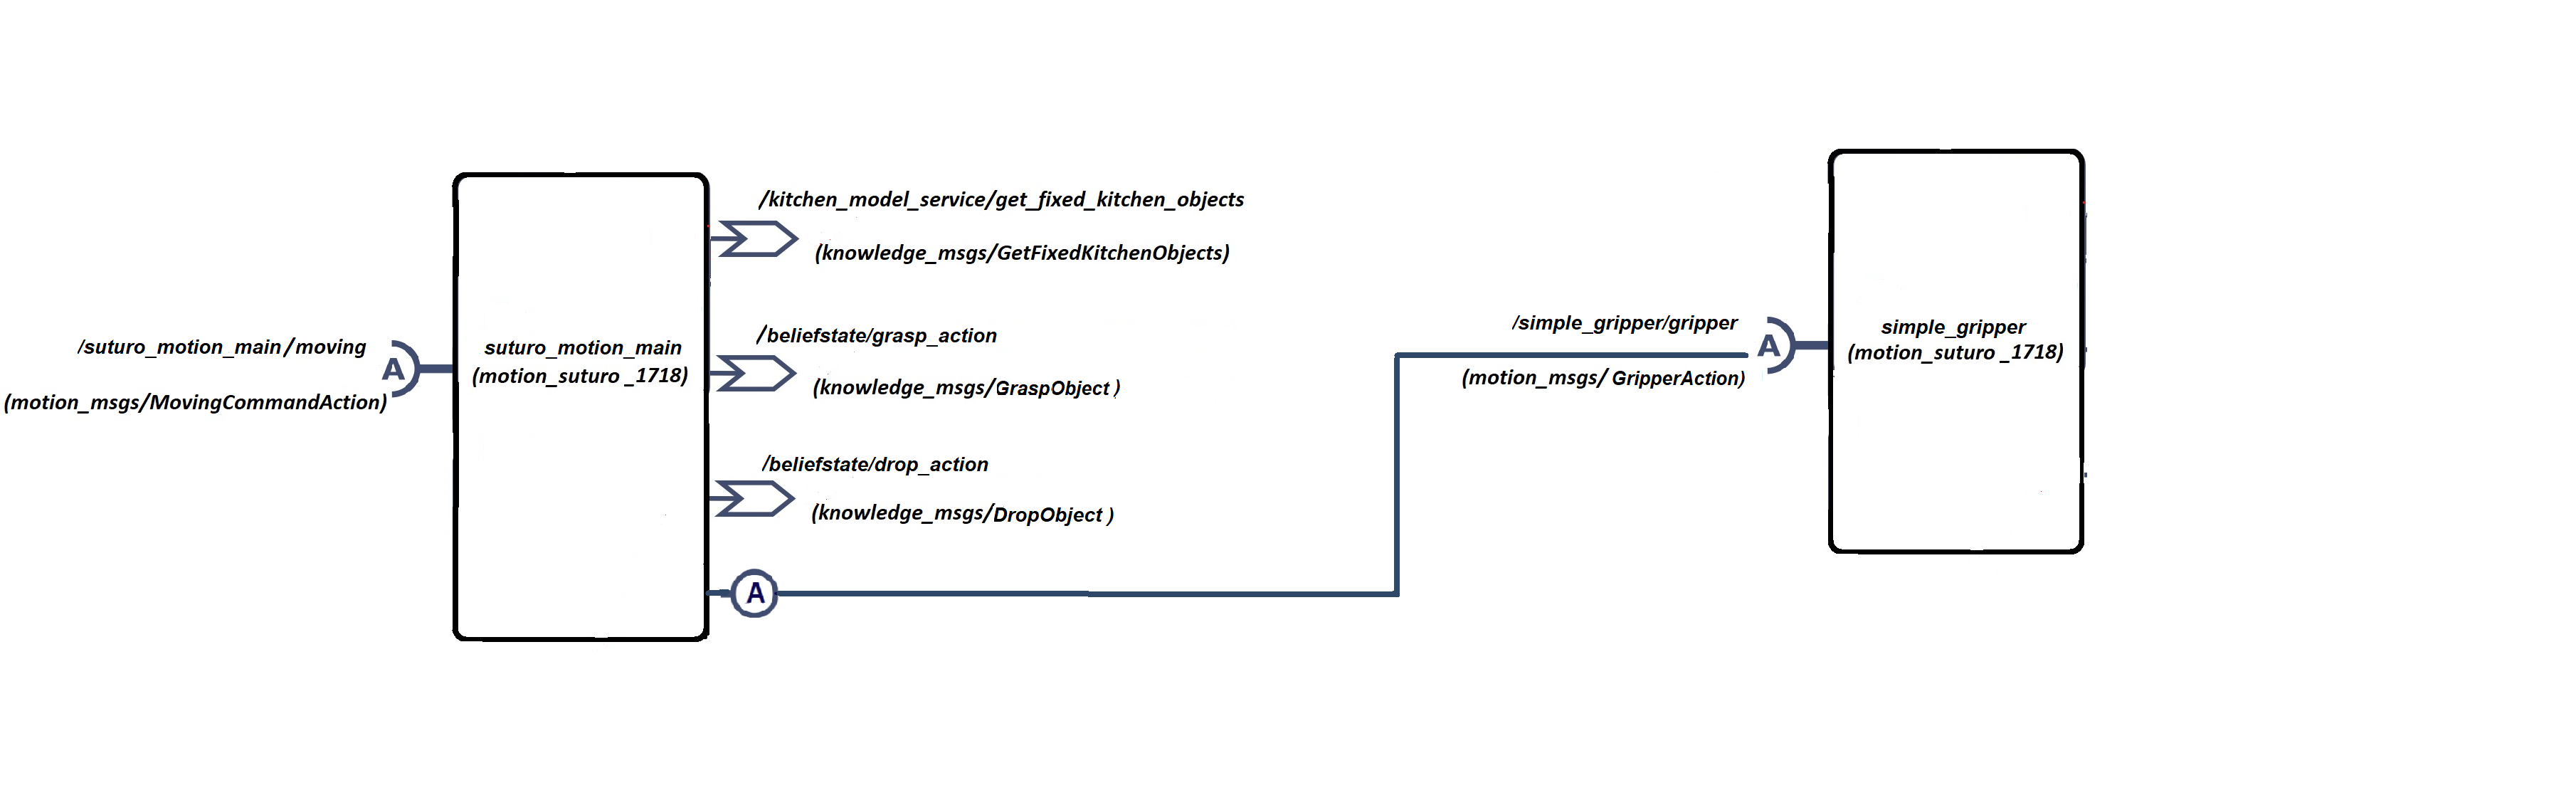
\includegraphics[width=\textwidth]
        {img/Architekturbild.png}
        \caption{\label{fig:motion_node} Architektur des Teilsystems der Gruppe 'Motion'}}
\end{figure}

\subsection{Übersicht des Teilsystems}
\chapterauthor{Roman Haak}
Die Untergruppe '\textit{Motion}' ist für das Bewegen verschiedener "Körperpartien" des Roboters zuständig.\\
Dabei wurde das Fahren des Roboters bis zu dem jetzigen Meilenstein von der Untergruppe '\textit{Planning}' übernommen, wird
in Zukunft aber von '\textit{Motion}' übernommen.\\
Das Bewegen der anderen, zum Erfüllen der Zielsetzung des Meilensteins 2 benötigten, Teile des Roboters, also Arm und Endeffektor (\textit{Gripper}) wurden 
von der Gruppe '\textit{Motion}' übernommen.\\

In \textit{Abbildung 1} Bild sieht man die Architektur des Teilsystems der Gruppe '\textit{Motion}'. Dabei gibt zwei Knoten '\textit{suturo\_motion\_main}' und '\textit{simple\_gripper}'.\\
Der Knoten '\textit{suturo\_motion\_main}' ist für das Verarbeiten eingehender Kommandos zum Bewegen der Arme bzw. eines Endeffektors zuständig. Dabei gibt es Kommandos für das Fahren der Arme in eine initiale Position, das Bewegen der Arme zu einer bestimmten Pose und das Umstubsen, Greifen oder Abstellen eines bestimmten Objektes mit einer bestimmten Pose.\\
Der Knoten '\textit{simple\_gripper}' wird dabei benutzt, um das Öffnen und Schließen des Endeffektors zu realisieren. Dieser Knoten wird von dem Hauptknoten '\textit{suturo\_motion\_main}' über einen Actionserver aufgerufen.\\

Im Folgenden werden die \textit{Schnittstellen}, der \textit{Ablauf} des Teilsystems, besonders \textit{hervorzuhebende} \textit{Algorithmen} und eine \textit{Installationsanleitung} beschrieben.

\subsection{Schnittstellen}
\subsubsection{'suturo\_motion\_main'}

\paragraph{1.3.1.1 Offered Actions}

\paragraph{1.3.1.1.1 MovingCommand}
\chapterauthor{Maximilian Bertram}
'\textit{/motion/moving}': \\
Vom Typ '\textit{motion\_msgs/MovingCommand}': \\
\begin{lstlisting}[caption={Definition der MovingCommandAction},captionpos=b]
#goal definition
geometry_msgs/PointStamped point_stamped
uint8 command
#Constants for command value
uint8 UNKNOWN=0
uint8 MOVE_STANDARD_POSE=1
uint8 MOVE_RIGHT_ARM=2
uint8 MOVE_LEFT_ARM=3
uint8 MOVE_RIGHT_GRIPPER=4
uint8 MOVE_LEFT_GRIPPER=5
---
#result definition
bool successful
uint8 status
#Constants for status value
uint8 SUCCESS=0
uint8 OUT_OF_RANGE=1
uint8 COLLISION=2
uint8 UNMANAGEBLE_ERROR=3
---
#feedback definition
#bool finished
\end{lstlisting}
TODO: Namen?\\
'\textit{/motion/moving}': \\
Vom Typ '\textit{motion\_msgs/MovingCommand}': \\


\paragraph{1.3.1.2 Called Actions}
- simple gripper/gripper hier
\paragraph{1.3.1.3 Offered Services}
- hier nichts
\paragraph{1.3.1.4 Called Services}
\chapterauthor{Roman Haak}
'\textit{/kitchen\_model\_service/get\_fixed\_kitchen\_objects}': \\
Dieser Service wird beim Initialisieren unseres Programms aufgerufen. Hierüber werden die Abmessungen der Objekte der IAI-Küche in die \textit{PlanningScene} geladen, damit der Roboter sich nur kollisionsfrei bewegt(siehe \textit{Kapitel 1.2.2}, Abschnitt zur '\textit{planning\_scene}').\\
Die Objekte sind dabei durch eine Höhe, Breite und Länge als \textit{Box-Collider} definiert.

- hier noch grasp\_action und drop\_action


\subsubsection{'simple\_gripper'}
\paragraph{1.3.2.1 Offered Actions}
\begin{lstlisting}[caption={Definition der GripperAction},captionpos=b]
#goal definition
#position of the space between the grippers in meters
float64 position
#force in newton (default =  20)
float64 effort
#which grpper to open/closed
uint8 gripper
#Constants for the gripper value
uint8 UNKNOWN=0
uint8 LEFT=1
uint8 RIGHT=2
---
#result definition
bool successful
---
#feedback definition
#bool finished
\end{lstlisting}
\paragraph{1.3.2.2 Called Actions}
-nichts
\paragraph{1.3.2.3 Offered Services}
-nichts
\paragraph{1.3.2.4 Called Services}
-nichts

\subsection{Ablauf}
\chapterauthor{}

\subsection{Besonderheiten/Besondere Algorithmen}
\chapterauthor{}

\subsection{Installationsanleitung}
\chapterauthor{}



\end{document}
